% =========================================================================
% Evaluating BFS Algorithms on Colored Balls in Colored Tubes
% -------------------------------------------------------------------------
% AAAI two-column style (classic AAAI Press LaTeX Template). On Overleaf,
% open the "AAAI Press LaTeX Template" as a template so that aaai.sty,
% aaai.bst, times.sty are present, then replace the main .tex with this file
% and add references.bib alongside it.
%
% Content corrected against the implementation and the recorded dataset in
% this repository. Points where the text was changed carry a % [FIX n] note
% so each correction can be traced back to the code or to RESULTS.md.
% =========================================================================

\documentclass[letterpaper]{article}
\usepackage{aaai}
\usepackage{times}
\usepackage{helvet}
\usepackage{courier}
\usepackage{graphicx}
\usepackage{amsmath}
\usepackage{amssymb}
% hyperref rather than url, so the repository link is clickable in the PDF.
% Loaded last, which is what hyperref wants, and with hidelinks so the anchor
% gets no colored box in print. It supersedes the url package and still
% provides \url. If a venue's style files reject hyperref, reverting this one
% line to \usepackage{url} degrades gracefully: the link still typesets, it
% just stops being clickable.
\usepackage[hidelinks]{hyperref}
\frenchspacing
\setlength{\pdfpagewidth}{8.5in}
\setlength{\pdfpageheight}{11in}

\nocopyright

\pdfinfo{
/Title (Evaluating Best-First Search Algorithms on Colored Balls in Colored Tubes)
/Author (Lea Galuk, Shahaf Harari)
}

\setcounter{secnumdepth}{0}

% [FIX 14] Retitled. "BFS" in the title collided with breadth-first search, which
% is one of the seventeen configurations evaluated. BFS now abbreviates best-first
% search only, and is spelled out here so the title carries no ambiguity; the
% breadth-first configuration is named \texttt{bfs}.
\title{Evaluating Best-First Search Algorithms on Colored Balls in Colored Tubes \\[4pt]
\large Search in Artificial Intelligence 26}

\author{
Lea Galuk\\
{\rm Ben-Gurion University of the Negev, Israel}\\
{\rm leashmil@post.bgu.ac.il}
\And
Shahaf Harari\\
{\rm Ben-Gurion University of the Negev, Israel}\\
{\rm shhara@post.bgu.ac.il}
}

\begin{document}

\maketitle

% [FIX 1] Domain description corrected. The implemented domain has NO per-tube
% color restriction: environments/BallSort.h states "There is deliberately NO
% color matching and NO per-tube color restriction", and GetActions generates
% every (source, dest) pair with a non-empty source and a non-full destination.
% [FIX 5] RSCBT is the paper's problem variant (their Definition 2); the solver
% is their Algorithm 1.
% [FIX 8] Effect size stated once, as the measured factor of 619.
% [FIX 9] "among the uninformed algorithms" dropped: A* with the misplaced-ball
% heuristic is informed and also fails by out-of-memory.
\begin{abstract}
We present an empirical evaluation of classical single-agent search algorithms on the colored-balls-in-colored-tubes puzzle, the variant of the ball-sorting puzzle studied by Althaus et al. (2025) in which each color has a designated goal tube and a single uncolored reserve tube supplies the only working space. We implement 17 algorithm configurations on the HOG2 search framework, spanning uninformed search (breadth-first search, bidirectional search, frontier search, iterative-deepening depth-first search, and Dijkstra's algorithm), optimal heuristic-guided search (A* and IDA*, each paired with a simple misplaced-ball heuristic and with the directed feedback vertex set bound of Althaus et al.), bounded-suboptimal and greedy search (weighted A* and greedy best-first search), and the search procedure of the base paper, together with a symmetry-reduction ablation and a 16-thread parallel variant. Across 660 reproducibly generated instances spanning 22 parameter cells of varying difficulty, for 11,220 total algorithm-instance runs, we find that heuristic quality is the dominant factor in search efficiency: replacing the misplaced-ball heuristic with the directed feedback vertex set bound reduces median node expansions by a factor of 619, more than two orders of magnitude, and raises coverage close to 100 percent. The base paper's own procedure matches this coverage but explores substantially more nodes than best-first search under the identical bound, indicating that its practical value lies in parallelizability rather than single-threaded search efficiency. Bounded suboptimality yields little benefit until weights are large enough to noticeably sacrifice solution quality, and the failure modes of the remaining algorithms follow their space complexity exactly. These results establish a systematic empirical baseline for search on this puzzle variant.
\end{abstract}

% =========================================================================
\section{Introduction}

Heuristic search lies at the core of artificial intelligence's approach to
problem solving in large, structured state spaces. Classical algorithms
such as breadth-first search, depth-first search, and their informed
counterparts (A*, IDA*) were developed and refined using single-agent
combinatorial puzzles as controlled, well-understood testbeds
\cite{hart1968,korf1985,russell2020}. Puzzles such as the sliding-tile
puzzle, Rubik's Cube, and Sokoban have historically served this purpose
because they combine an intuitive formulation with a state space whose
size, branching factor, and goal structure can be analyzed precisely
\cite{ratner1986,korf1997,culberson1998,junghanns2001}.

A more recent addition to this family of benchmark problems is the
ball-sorting puzzle, in which colored balls are stacked in tubes and must
be rearranged, one move at a time, until every tube holds balls of a
single color. Beyond its popularity as a casual mobile game, the puzzle
has attracted theoretical interest: it has been shown to be NP-complete
\cite{ito2023}, and its combinatorial structure has proven rich
enough to support cryptographic protocols such as zero-knowledge proofs
\cite{ruangwises2023}.
% [FIX 1] Corrected description of what "colored tubes" means in this model.
Althaus et al.\ \cite{althaus2025} study a formulation in which the tubes
themselves are colored: over $c$ colors there are $c+1$ tubes of equal
height, one designated goal tube per color plus a single uncolored reserve,
and every colored tube begins full. Placement itself remains unrestricted,
so the top ball of any non-empty tube may be moved onto any tube that is
not full. The difficulty comes from the capacity structure rather than from
a placement rule: one tube's worth of empty space is the only slack
available for the entire rearrangement. This model is a natural abstraction
of sorting, storage, and recycling tasks in which destination containers
are labeled and buffer space is scarce.

Studying this puzzle is motivated by two complementary needs.
First, before any heuristic or learned search method can be meaningfully
evaluated, a reliable and well-understood baseline is required; blind
search algorithms such as breadth-first search provide exactly this kind of
ground truth, since they are guaranteed to find a shortest solution (in
terms of number of moves) whenever the state space is fully explored.
Second, the formulation is recent enough that, to the best of our
knowledge, no systematic empirical study of how basic uninformed search
behaves on it, in terms of runtime, memory consumption, and state-space
growth, has yet been published. Understanding this baseline behavior is a
necessary first step toward designing and evaluating stronger heuristics
for the problem.

The objective of this work is therefore to implement and empirically
evaluate a broad family of classical single-agent search algorithms on the
colored-balls-in-colored-tubes formulation of Althaus et al.\
\cite{althaus2025}. The organizing template is best-first search (BFS), in
which a node is repeatedly selected for expansion from the search frontier
according to an evaluation function $f(n)$ \cite{pearl1984,russell2020}.
Throughout this paper BFS abbreviates best-first search and nothing else.
Breadth-first search is a distinct algorithm, one of the seventeen
configurations evaluated below; it is written out in full wherever it appears
in prose, and the configuration itself is named \texttt{bfs}.
% [FIX 14] The family is no longer described as uniformly best-first: IDDFS,
% IDA* and the base paper's Algorithm 1 are not best-first algorithms, and the
% Results section says as much about Algorithm 1.
Several members of the family we evaluate are deliberately not best-first:
the iterative-deepening algorithms explore depth-first under a bound, and
the base paper's own procedure expands in breadth-first layer order. These
are included precisely because they trade search order for space, which is
what the comparison is meant to expose. The family thus ranges from plain
breadth-first search, bidirectional search, frontier search,
iterative-deepening search, and Dijkstra's algorithm, through A*, IDA*,
weighted A*, and greedy best-first search, to the base paper's own solver.
We characterize the behavior of these algorithms, including solution
optimality, runtime, and state-space growth, across instances of varying
size and difficulty, so that the resulting analysis can serve as a baseline
against which future search-based approaches to this puzzle can be
compared.
% [FIX 12] One-line pointer to the repository. The build instructions, the file
% map and the reproducibility notes live in the repository's README, not here.
Our code and results can be found at
\url{https://github.com/lea-shmil/ballsort-hog2}.

% =========================================================================
\section{Related Work}

\subsection{Search Algorithms and Puzzle Benchmarks}

The use of combinatorial puzzles to study search algorithms dates back to
the foundational work on informed search, most notably the A* algorithm
\cite{hart1968}, which remains the standard reference for optimal,
heuristic-guided search, and Dijkstra's uniform-cost algorithm
\cite{dijkstra1959}, which is equivalent to A* with a zero heuristic and
expands nodes strictly in order of accumulated path cost. Breadth-first
search, the simplest complete and optimal uninformed instantiation in
unit-cost domains, expands nodes in order of increasing depth, but its
memory requirements grow exponentially with solution depth. Two classical
remedies address this limitation: Pohl's
bidirectional search \cite{pohl1971} grows two frontiers simultaneously
from the start and goal states until they meet, cutting the number of
nodes that must be expanded, and Korf et al.'s frontier search
\cite{korf2005} discards expanded nodes and retains only the current
search frontier and the layer immediately behind it, substantially
reducing peak memory. Korf's iterative-deepening framework
\cite{korf1985} takes a different approach, combining the linear space
complexity of depth-first search with the completeness and optimality of
breadth-first search through repeated depth-limited passes
(iterative-deepening DFS, or IDDFS); when the same idea is paired with an
admissible heuristic instead of a fixed depth bound, it yields IDA*, an
optimal alternative to A* that avoids storing open and closed lists
entirely.

When strict optimality is not required, bounded-suboptimal and purely
greedy variants trade solution quality for speed. Weighted A*
\cite{pohl1970} inflates the heuristic term in the evaluation function
$f(n) = g(n) + w \cdot h(n)$ to bias the search more aggressively toward
the goal at the cost of a bounded loss in optimality, while greedy
best-first search \cite{doran1966} orders expansions purely by $h(n)$,
ignoring accumulated cost altogether. Ratner and Warmuth
\cite{ratner1986} showed that finding a \emph{shortest} solution for the
$n \times n$ generalization of the 15-puzzle is NP-hard, which helps
explain why blind search alone becomes intractable as puzzle instances
scale and motivated the design of strong admissible heuristics. Building
on this line of work, Korf \cite{korf1997} and Culberson and Schaeffer
\cite{culberson1998} introduced pattern databases, precomputed admissible
heuristics that made optimal solving of Rubik's Cube and similarly
structured puzzles practical, and Junghanns and Schaeffer
\cite{junghanns2001} showed that domain-specific pruning and macro moves
were necessary to make progress on Sokoban, whose branching factor and
solution depth make blind and naively informed search infeasible.

% [FIX 3] The bound is a sum of a per-ball counting term and a DFVS term, not
% the DFVS size alone (see include/dfvs_bound.h, PaperLowerBound).
% [FIX 5] RSCBT names the problem variant (their Definition 2). The solver is
% their Algorithm 1, a breadth-first branch and bound. The draft's expansion
% "constraint-based tree search" is not supported by the paper or the code.
Directly relevant to the present project, Althaus et al.
\cite{althaus2025} introduce an admissible lower bound for this puzzle that
combines a per-ball counting argument with a directed feedback vertex set
(DFVS) term, together with a solver, their Algorithm 1, that searches the
configuration space breadth-first as a branch and bound under an ascending
bound, holding only three adjacent layers in memory and collapsing
color-permutation-equivalent configurations to a single representative.
Their Definition 2 names the restricted problem variant RSCBT; following
our implementation we use \texttt{rscbt} as the label for our
reimplementation of their Algorithm 1 on that problem. Together with the
classical algorithms above, these contributions form the basis of the
search methods evaluated in this work: uninformed search (breadth-first
search, bidirectional breadth-first search, frontier breadth-first search,
IDDFS, and Dijkstra), optimal heuristic-guided search (A* and IDA*, each
paired with a simple misplaced-ball heuristic as well as the DFVS-based
bound of \cite{althaus2025}), bounded-suboptimal and greedy search
(weighted A* and greedy best-first search), and their Algorithm 1 in three
configurations: with symmetry reduction, without it, and with the layer
expansion parallelized across 16 threads.

\subsection{Ball- and Water-Sorting Puzzles}

A more specific line of work studies sorting puzzles in which colored
units (balls or water) are stacked inside bins or tubes that behave like
stacks. Ito et al.\ \cite{ito2023} formalize both the ball-sort and
water-sort puzzles, prove that the two puzzle families are equivalent from
the viewpoint of solvability, show that a solution (when one exists)
always has polynomial length (placing the puzzle in NP), and establish
NP-completeness of finding a solution even when only two colors are involved
(their Theorem 9). They also identify polynomial-time solvable special cases,
notably instances in which every tube has capacity two, where a shortest
sorting sequence can be found in linear time (their Theorems 13 and 14). The
two-color hardness result is worth stating precisely here, because it rules out
any hope that a small palette makes the problem easy: the difficulty of this
puzzle family comes from the stacking discipline and the scarcity of free
space, not from the number of colors.
% [FIX 11] Both restrictions verified against the paper body and restored with
% their theorem numbers. An earlier revision of this file removed them on the
% grounds that the published abstract does not state either one; that was
% over-cautious, since the abstract only says "NP-complete" and "for some
% special cases, we give polynomial-time algorithms" while Theorem 9 and
% Theorems 13-14 give exactly the restrictions the original text claimed.
Ruangwises \cite{ruangwises2023} builds on the same puzzle
definition to design a physical zero-knowledge proof protocol for the ball
sort puzzle, demonstrating that its state space is combinatorially rich
enough to support non-trivial cryptographic reasoning about knowledge of a
solution without revealing that solution. These works, however, focus on
complexity-theoretic and cryptographic characterizations of the puzzle
rather than on the empirical performance of concrete search algorithms
that actually find solutions.

\subsection{Positioning of This Project}

Althaus et al.\ \cite{althaus2025} supply the problem formulation, the
instance-generation procedure, the parameter grid, the reported metric set,
and the lower bounds that this project builds upon directly. While the
broader search literature has extensively studied uninformed and heuristic
search on structurally related puzzles, such as the 15-puzzle, Rubik's
Cube, and Sokoban
\cite{ratner1986,korf1985,korf1997,culberson1998,junghanns2001}, and the
ball/water-sorting literature has focused mainly on complexity results and
cryptographic applications \cite{ito2023,ruangwises2023}, a systematic,
empirical evaluation of the classical search family, from uninformed
instantiations such as breadth-first search to heuristic-guided,
bounded-suboptimal, and domain-specific variants, on the
colored-balls-in-colored-tubes model has not, to our knowledge, yet been
reported. This project addresses that gap: by evaluating this family
directly on the model of \cite{althaus2025}, it aims to provide the
systematic baseline that connects the theoretical complexity results of
\cite{ito2023} with the practical algorithm-design goals pursued in
\cite{althaus2025}, and to lay the groundwork for a future comparison with
learned and other informed solvers on this specific puzzle.

% =========================================================================
\section{Methods}

\subsection{Domain and Problem Instances}

We adopt the colored-balls-in-colored-tubes formulation exactly as defined by
Althaus et al.\ \cite{althaus2025}. A problem instance over $c$ colors
consists of $c+1$ tubes of uniform height $h$: an uncolored reserve tube
$T_0$ and one goal tube $T_i$ for each color $i \in \{1, \dots, c\}$. The
start state has $T_0$ empty and every colored tube full. A
legal move $(i,j)$ transfers the top ball of tube $i$ onto tube $j$,
provided tube $i$ is non-empty and tube $j$ is not full; there is no
color-matching restriction and no per-tube color restriction, so any top
ball may be placed on any non-full tube. The goal state has the reserve
empty and every tube $T_i$ filled entirely with balls of color $i$. Because
every full-tube start state with exactly $h$ balls of each color is
guaranteed solvable, generated instances require no solvability filtering.

Instances are generated following the uniform shuffling procedure of
Althaus et al.\ (their Section 7): a flat multiset of $c \times h$ color
tokens ($h$ copies of each color) is uniformly shuffled and sliced into $c$
contiguous segments of length $h$, filling the colored tubes from bottom to
top while leaving the reserve empty. Each instance is deterministically
seeded from the tuple of global seed, height, number of tubes, and instance
index, so the instance set is exactly reproducible and can be regenerated on
demand rather than stored. Generation includes a color count check prior to
writing and a round trip read-back verification after writing.

\subsection{Parameter Grid and Instance Set}

Parameter configurations are indexed as $h \times (c+1)$, following the
paper's cell naming convention; for example, cell $4 \times 8$ denotes
height $h=4$ over 8 total tubes ($c=7$ colors). We transcribe the full
53-cell grid published by Althaus et al., but our perfect state hash packs a
state into a fixed-width 64-bit integer, which requires
$(c+1)^{h(c+1)} < 2^{64}$ and admits only 29 of the 53 cells; in particular
the paper's own headline cell, $4 \times 8$, cannot be encoded and is out of
reach for the algorithms compared here.

% [FIX 2] The core set spans THREE tiers (A, B, C), not four. CoreGridCells()
% in include/instance_gen.h skips both kTierTrivial and kTierD; the trivial
% tier is defined in order to be excluded.
From the 29 encodable cells we select a core comparison set of 22 cells,
tiered on the exact reachable configuration count
$N = \frac{(h+c)! \, (hc)!}{c! \, (h!)^{c+1}}$ (also from the paper). The
core set spans three tiers: tier A ($N \in [10^3, 10^5]$, where
linear-space depth-limited search still finishes), tier B
($N \in [10^5, 10^8]$, the largest cells the memory-bounded optimal
algorithms can attempt), and tier C ($N \in [10^8, 10^{11}]$, reachable
only by heuristic-guided or bounded-suboptimal search). Cells below tier A
($N < 10^3$) are excluded as trivial, since every algorithm solves them
instantly and they separate nothing, and cells above tier C
($N \geq 10^{11}$) are excluded as beyond reach with the present heuristic.
For each core cell we draw 10 instances under each of three independent
global seeds, for 30 instances per cell and 660 problem instances in total.
A minimum simple lower bound filter of 1 excludes the rare already-solved
shuffle.

\subsection{Algorithms and Implementation}

All algorithms are implemented against the HOG2 search framework
\cite{sturtevant2012} in a headless, single-threaded configuration, compiled
in release mode. We evaluate 17 algorithm configurations, organized into
four groups.

\emph{Uninformed search} ($h \equiv 0$, all optimal): breadth-first search,
bidirectional breadth-first search, and Dijkstra's algorithm (A* with
$h=0$) use HOG2's built-in implementations; frontier search and
iterative-deepening depth-first search (IDDFS, also called DFID) are our
own implementations, written after finding that the corresponding HOG2
headers do not terminate correctly on this domain on the framework's
current branch (frontier search never calls the goal test, and IDDFS's own
goal test is disabled).

% [FIX 3] h_DFVS = BasicLowerBound + DFVSLowerBound, and the graph construction
% follows the authors' released code rather than the per-color feedback arc set
% exposition in their Section 5. Both points were wrong or missing before.
\emph{Heuristic-guided optimal search}: A* and IDA* are each run twice,
once with a simple misplaced-ball count heuristic $h_{mis}$ (the number of
balls not in their goal tube), and once with the lower bound
$h_{DFVS}$ of Althaus et al.\ \cite{althaus2025}. That bound is the sum of
two terms. The first is a per-ball counting bound: a ball already in final
position contributes $0$, a ball of color $i$ sitting in tube $i$ above a
foreign ball contributes $2$ because it must leave and return, and any
other ball contributes $1$. The second is a directed feedback vertex set
term, the size of a minimum feedback vertex set of a graph with one vertex
per tube slot, less those set members that are home-tube balls out of final
position and are forced into every minimum set by self-loops. We compute
the minimum exactly with our own branch-and-bound solver rather than the
PACE solver the authors call. One reproducibility note is worth recording:
the authors' Section 5 motivates the bound through a feedback arc set
problem on a graph with one vertex per \emph{color}, whereas their released
implementation builds the per-slot graph described above and solves DFVS on
it directly. We follow the implementation, since it is what produced their
published numbers. On our instances the bound is admissible against
breadth-first ground truth, consistent (the largest $|h(n)-h(n')|$ over all
33,600 states of cell $3 \times 4$ is 1, so A* requires no reopening), and
strictly dominates the per-ball bound alone.

\emph{Bounded-suboptimal and greedy search}: weighted A* with
$f(n) = g(n) + w \cdot h_{DFVS}(n)$ is evaluated at
$w \in \{1.005, 1.01, 1.05, 1.1\}$, and greedy best-first search orders
expansions purely by $h_{DFVS}(n)$, corresponding to the $w \to \infty$ end
of the same family. The weights sit just above 1 because that is where the
interesting region lies: in a preliminary pass, $w = 1.25$ already returned
the optimal length on more than half of its instances.

% [FIX 5] "the base paper's own solver" rather than "RSCBT, the algorithm".
\emph{The base paper's own solver}: Algorithm 1 of Althaus et al.\ is
reimplemented from their description as a breadth-first branch and bound
over configurations, retaining only three adjacent layers at a time and
filtering successors against an upper bound $\mu$ with $h_{DFVS}$; because
Algorithm 1 is a decision procedure, the optimal solution length is found
by sweeping $\mu$ upward from the root bound, the first success being
optimal. We evaluate it with color-permutation symmetry reduction
(\texttt{rscbt}), without it (\texttt{rscbt-nosym}), and as a 16-thread
parallel implementation (\texttt{rscbt-par}); single-threaded execution is
used elsewhere so that the comparison is not confounded by thread count.

\subsection{Experimental Protocol and Metrics}

All 660 core instances are run under all 17 configurations, for 11,220
attempted algorithm-instance pairs. Every run executes as a single process
on one of twelve homogeneous compute nodes of a shared cluster (identical
AMD EPYC 7702P CPUs at the same clock frequency), so that wall-clock
comparisons are not confounded by hardware heterogeneity; the CPU model is
logged with every result row and checked automatically. Each run repeats
its search three times and reports the median wall-clock time, to reduce
scheduler jitter; because every algorithm here is deterministic, only
wall-clock time benefits from repetition, since node counts and solution
lengths are identical across repeats of the same instance. Each run is
allotted 32 GB of memory and a 3,600 second process timeout; since the
timeout bounds the whole three-repeat process rather than a single search,
the effective per-search budget is close to 1,200 seconds.
% [FIX 10] The reported dataset used a flat 32 GB. Recorded so the number is
% not silently at odds with the repository's current sweep configuration.
The reported dataset was collected with a flat 32 GB allocation per run;
the memory budget has since been raised to 60 GB for the closed-list
searches, which by measurement would recover on the order of 28 additional
completed runs, all in cells $12 \times 3$ and $13 \times 3$. Node counts
and solution lengths are independent of both limits.

For each algorithm-instance pair we record the four metrics reported by
Althaus et al.\ (their Figure 6): median wall-clock runtime, peak resident
memory, the maximum number of states held in memory during search, and
solution length. We additionally record nodes expanded and generated
(hardware-independent measures of state-space exploration), whether the run
completed within its resource limits, the suboptimality ratio for
non-optimal algorithms, the root heuristic estimate, and the iteration
count for iterative algorithms (IDDFS, IDA*, and the sweep over $\mu$).

% [FIX 15] The contract as implemented (OPTIMAL_ALGORITHMS in
% slurm/aggregate_results.py) covers twelve configurations, including all three
% Algorithm 1 variants, not the seven the draft claimed.
Before reporting results we verify a correctness contract: all twelve
configurations that are guaranteed optimal (breadth-first search,
bidirectional breadth-first search, frontier search, IDDFS, Dijkstra's
algorithm, A* and IDA* with either heuristic, and the three variants of
Algorithm 1) must return the same solution length on every instance they
solve; weighted A* must never exceed its theoretical $w$-bound, and greedy
best-first search must never return a length below optimal; and
\texttt{rscbt} and \texttt{rscbt-par}, which are deterministic by
construction, must expand identical node counts on every instance.

% =========================================================================
\section{Experimental Results}

\subsection{Correctness and Determinism}

The correctness contract described in Methods holds without exception
across all 660 core instances: the twelve optimality-guaranteed
configurations never disagree on solution length; no weighted A* run
exceeds its theoretical $w$-bound; and \texttt{rscbt} and
\texttt{rscbt-par} expand byte-identical node counts on every one of the
660 instances, confirming that the parallel implementation's layer merging
is exactly deterministic in thread count. Every recorded timing also ran on
the same CPU model, so the runtime comparisons below are not confounded by
hardware.

\subsection{Coverage and Runtime}

Of the 11,220 attempted runs, 9,828 completed within the resource limits
and 1,392 were terminated. Table~\ref{tab:coverage} summarizes coverage
(the fraction of the 660 core instances solved) and median runtime by
algorithm, and Figure~\ref{fig:coverage} shows the same coverage broken down
by how the terminated runs died. A* with the DFVS bound solves every instance in a few
milliseconds; Algorithm 1 in all three configurations and the weighted A*
and greedy configurations likewise reach 100\% coverage.
% [FIX 4] The draft claimed the uninformed algorithms range from 72.7% down to
% 23.9%, contradicting its own table: bidirectional BFS is uninformed and
% reaches 99.7%.
Among the remaining algorithms, bidirectional breadth-first search is the
one uninformed method that stays competitive, at 99.7\%, because its two
frontiers meet near the middle and it never has to hold a full layer of the
deep end. The other four uninformed algorithms fall well short, from 72.7\%
for breadth-first search down to 23.9\% for IDDFS, and A* and IDA* with the
weaker misplaced-ball heuristic sit at 96.4\% and 56.8\% respectively.

\begin{table}[t]
\centering
\footnotesize
\caption{Coverage and median runtime over the 660 core instances.}
\label{tab:coverage}
\begin{tabular}{lccc}
\hline
Algorithm & Solved & Coverage & Runtime (s) \\
\hline
\texttt{astar-paper} & 660 & 100.0\% & 0.0036 \\
\texttt{rscbt} & 660 & 100.0\% & 0.0430 \\
\texttt{rscbt-nosym} & 660 & 100.0\% & 0.0310 \\
\texttt{rscbt-par} & 660 & 100.0\% & 0.0410 \\
\texttt{wastar-1.005} to \texttt{-1.1} & 660 & 100.0\% & 0.0012--0.0047 \\
\texttt{greedy} & 660 & 100.0\% & 0.0012 \\
\texttt{bibfs} & 658 & 99.7\% & 0.1200 \\
\texttt{idastar-paper} & 655 & 99.2\% & 0.0050 \\
\texttt{astar-misplaced} & 636 & 96.4\% & 0.0980 \\
\texttt{bfs} & 480 & 72.7\% & 1.5480 \\
\texttt{frontier-bfs} & 467 & 70.8\% & 0.9980 \\
\texttt{dijkstra} & 459 & 69.5\% & 1.7830 \\
\texttt{idastar-misplaced} & 375 & 56.8\% & 0.1950 \\
\texttt{iddfs} & 158 & 23.9\% & 2.0770 \\
\hline
\end{tabular}
\end{table}

% [FIG] Produced by slurm/plot_results.py from results/per_cell.csv and the
% KILLED lines in logs/sweep/*.out. Regenerate rather than editing by hand.
\begin{figure}[t]
\centering
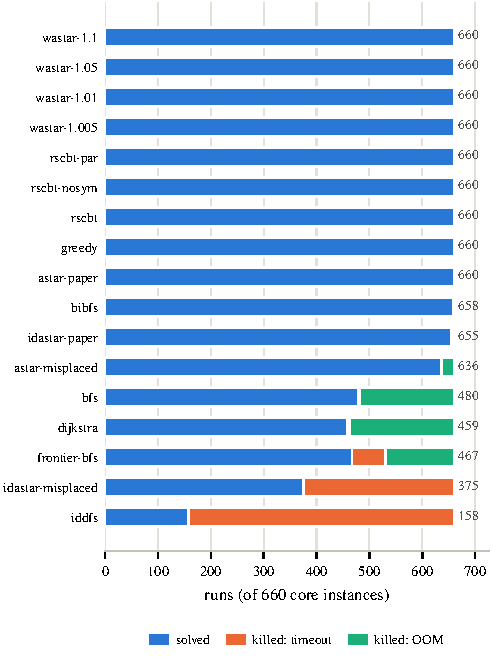
\includegraphics[width=\columnwidth]{figures/fig_coverage}
\caption{Run outcomes per algorithm over the 660 core instances, sorted by
coverage. Separating the two ways a run can be killed shows the space-complexity
split directly: the linear-space searches (\texttt{iddfs},
\texttt{idastar-\-misplaced}, \texttt{idastar-paper}) run out of clock and never
out of memory, while every out-of-memory failure belongs to a search that keeps a
closed list.}
\label{fig:coverage}
\end{figure}

\subsection{Effect of Heuristic Quality}

Table~\ref{tab:heuristic} isolates the effect of the heuristic itself by
comparing A* and IDA* under $h_{mis}$ and $h_{DFVS}$. Replacing the
misplaced-ball count with the DFVS-based bound reduces the median number of
nodes expanded from 61,934 to 100, a factor of 619, and raises coverage
from 96.4\% to 100.0\% for A* and from 56.8\% to 99.2\% for IDA*. No other
factor examined in this study produces an effect of comparable size, which
indicates that heuristic quality, not the choice of search order, is the
dominant determinant of search efficiency on this domain.
Figure~\ref{fig:expansions} shows how that difference behaves as the state
space grows: across the whole core grid the searches guided by $h_{DFVS}$
grow markedly more slowly than $N$, while the uninformed searches track it
directly, so the gap between the two heuristics widens with cell size rather
than staying at the constant factor a single median suggests.
% [FIX 7] The 100 versus 116 difference is now stated explicitly rather than
% left for the reader to reconcile across tables.
The expansion medians in Table~\ref{tab:heuristic} are taken over the 636
instances that both A* variants solve, so that the comparison is
like-for-like; over all 660 instances the median for A* with $h_{DFVS}$ is
116, which is the figure used in Tables~\ref{tab:rscbt}
and~\ref{tab:suboptimal}. The coverage columns are over all 660 instances
in both rows.

\begin{table}[t]
\centering
\footnotesize
\caption{Heuristic quality versus search efficiency. Expansions are medians
over the 636 instances solved by both A* variants; coverage is over all 660
instances.}
\label{tab:heuristic}
\begin{tabular}{lccc}
\hline
Heuristic & Med. Expanded & Cov. (A*) & Cov. (IDA*) \\
\hline
Misplaced balls ($h_{mis}$) & 61{,}934 & 96.4\% & 56.8\% \\
DFVS bound ($h_{DFVS}$) & 100 & 100.0\% & 99.2\% \\
\hline
\end{tabular}
\end{table}

% [FIG] Produced by slurm/plot_results.py from results/per_cell.csv.
\begin{figure*}[t]
\centering
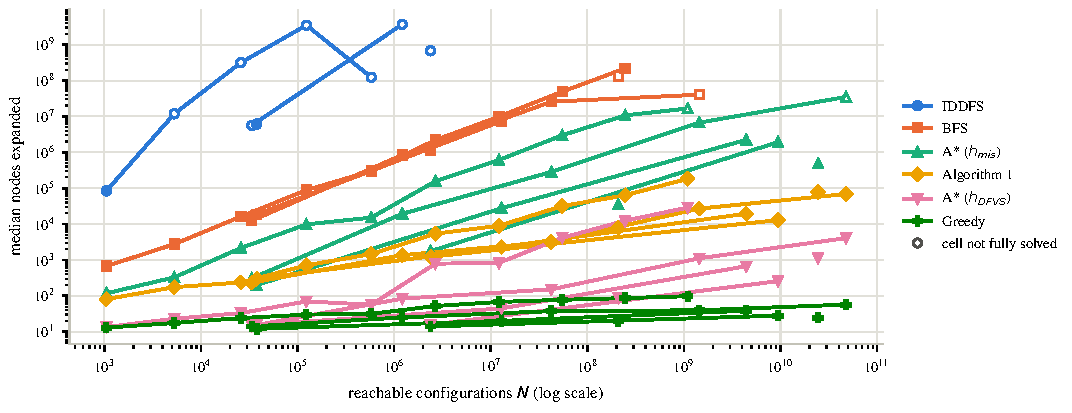
\includegraphics[width=\textwidth]{figures/fig_expansions_vs_states}
\caption{Median nodes expanded against the exact reachable configuration count
$N$, over the 22 core cells, for one representative algorithm per class. Both
axes are logarithmic. Over the seven orders of magnitude of $N$ the grid spans,
the searches guided by $h_{DFVS}$ grow by two to three, and greedy best-first
search by about one, while breadth-first search grows roughly in proportion to
$N$, as an exhaustive search must, and iterative deepening faster still. The
uninformed series also stop early, at the cell where their budget runs out.
Line segments join
cells that share a tube count, within which raising the height raises $N$ and
the cost together; cells with different tube counts are not joined, since two
cells of similar $N$ but different shape are not comparable. Hollow markers mark
cells the algorithm did not solve completely, where the median is taken over the
solved instances only and therefore understates the true cost of the cell.}
\label{fig:expansions}
\end{figure*}

\subsection{The Base Paper's Algorithm}

Algorithm 1 reaches 100\% coverage, matching \texttt{astar-paper}, but it
is not competitive with best-first search under the same bound:
Table~\ref{tab:rscbt} shows a median of 2,687 nodes expanded for
\texttt{rscbt} against 116 for A* with $h_{DFVS}$, a factor of 23. This gap
is expected rather than a defect, since Algorithm 1 expands configurations
breadth-first, layer by layer under an ascending bound, rather than
ordering by $f(n)$, and can re-derive work across iterations that A* orders
away. Disabling color-permutation symmetry reduction
(\texttt{rscbt-nosym}) raises median expansions from 2,687 to 3,072, a
factor of 1.14, confirming that the reduction helps but is not the main
source of the overhead relative to best-first search.
% [FIX 6] rscbt's counts are over the symmetry-reduced quotient space, which
% include/rscbt.h notes "makes node counts incomparable with the other
% algorithms'". The strictly like-for-like comparison is rscbt-nosym.
Because symmetry reduction searches a quotient of the state space, the
strictly like-for-like comparison against A* is \texttt{rscbt-nosym}, which
widens the gap to a factor of 26 rather than narrowing it. The
16-thread implementation (\texttt{rscbt-par}) shows essentially no speedup
across all 660 instances (median $0.99\times$) because most instances
finish in well under a second and thread setup dominates, but restricted to
the 121 instances requiring more than one second of serial runtime it
achieves a median speedup of $2.82\times$ and a maximum of $7.67\times$.

\begin{table}[t]
\centering
\footnotesize
\caption{Node expansions under the identical DFVS bound, medians over all
660 instances.}
\label{tab:rscbt}
\begin{tabular}{lp{2.7cm}c}
\hline
Algorithm & Search strategy & Med. expanded \\
\hline
\texttt{astar-paper} & best-first ($f=g+h$) & 116 \\
\texttt{rscbt} & breadth-first, layer by layer, symmetry-reduced & 2{,}687 \\
\texttt{rscbt-nosym} & breadth-first, layer by layer, raw state space & 3{,}072 \\
\hline
\end{tabular}
\end{table}

\subsection{Suboptimal Search Trade-offs}

Table~\ref{tab:suboptimal} evaluates whether relaxing optimality with
weighted A* or greedy best-first search buys additional search-space
reduction. Because the DFVS bound is already tight enough that A* expands
only about 116 nodes per instance on median, weighted A* at small weights
($w \le 1.05$) returns the optimal solution on every instance
and reduces expansions negligibly; only at $w = 1.1$ does the count of
optimal solutions drop to 627/660 (95\%), with a mean suboptimality ratio
of 1.0017 and expansions falling to a median of 91.5, the one median here
that is not a whole number because 660 is even. Greedy best-first
search, the $w \to \infty$ end of the family, cuts median expansions to 31
(a factor of 3.74 relative to A*) but returns the optimal solution on
only 149/660 instances (23\%), with a mean suboptimality ratio of 1.416
and a worst case of 3.423. On this domain, therefore, bounded suboptimality
below $w=1.1$ buys nothing, while greedy search is a genuine
speed-quality trade-off rather than a free improvement.

\begin{table*}[t]
\centering
\footnotesize
\caption{Suboptimal search: solution quality versus node expansions.}
\label{tab:suboptimal}
\begin{tabular}{lcccc}
\hline
Algorithm & Mean ratio & Max ratio & Optimal found & Med. expanded \\
\hline
\texttt{astar-paper} ($w=1.0$) & 1.0000 & 1.000 & 660/660 (100\%) & 116 \\
\texttt{wastar-1.005} & 1.0000 & 1.000 & 660/660 (100\%) & 116 \\
\texttt{wastar-1.01} & 1.0000 & 1.000 & 660/660 (100\%) & 116 \\
\texttt{wastar-1.05} & 1.0000 & 1.000 & 660/660 (100\%) & 116 \\
\texttt{wastar-1.1} & 1.0017 & 1.050 & 627/660 (95\%) & 91.5 \\
\texttt{greedy} ($w=\infty$) & 1.4160 & 3.423 & 149/660 (23\%) & 31 \\
\hline
\end{tabular}
\end{table*}

\subsection{Failure Mode Analysis}

Re-examining the 1,392 terminated runs separates timeouts from
out-of-memory failures: 860 were timeouts and 532 were out-of-memory.
Table~\ref{tab:failure} shows this split follows algorithm class exactly as
predicted by space complexity: the linear-space searches (IDDFS, IDA* with
either heuristic) record zero out-of-memory failures and fail only by
timeout, while the closed-list searches (breadth-first search, Dijkstra's
algorithm, frontier search, bidirectional breadth-first search, A* with the
misplaced-ball heuristic) account for every out-of-memory failure.
Out-of-memory failures are confined to the largest core cells ($12\times3$,
$13\times3$, $2\times8$, $3\times6$, $4\times5$, $6\times4$, $7\times4$);
smaller cells that fail do so by timeout only. Neither
\texttt{astar-paper} nor any configuration of Algorithm 1 nor any
suboptimal configuration appears in the table, since none of them failed a
single run.

\begin{table}[t]
\centering
\footnotesize
\caption{Cause of termination among the 1,392 killed runs.}
\label{tab:failure}
\begin{tabular}{llcc}
\hline
Category & Algorithm & Timeout & OOM \\
\hline
Linear space & \texttt{iddfs} & 502 & 0 \\
 & \texttt{idastar-misplaced} & 285 & 0 \\
 & \texttt{idastar-paper} & 5 & 0 \\
Closed list & \texttt{frontier-bfs} & 63 & 130 \\
 & \texttt{dijkstra} & 3 & 198 \\
 & \texttt{bfs} & 2 & 178 \\
 & \texttt{astar-misplaced} & 0 & 24 \\
 & \texttt{bibfs} & 0 & 2 \\
\hline
\end{tabular}
\end{table}

% =========================================================================
\section{Conclusions}

This work implemented and empirically evaluated a broad family of
classical search algorithms, spanning uninformed search, heuristic-guided
optimal search, bounded-suboptimal and greedy search, and the base paper's
domain-specific solver, on the colored-balls-in-colored-tubes puzzle
of Althaus et al.\ \cite{althaus2025}. Across 11,220 runs over 660
reproducibly generated instances, three conclusions stand out.

% [FIX 8] Consistent with the measured factor of 619 throughout.
First, heuristic quality, not search order, is the dominant factor in this
domain: replacing a naive misplaced-ball count with the paper's DFVS-based
bound cuts median node expansions by a factor of 619, more than two orders
of magnitude, and raises coverage of the heuristic-guided algorithms close
to 100\%, an effect far larger than any difference among uninformed
algorithms or among bounded-suboptimal weights.

Second, the base paper's own algorithm is robust but not
search-efficient: it solves every core instance, matching the best
heuristic-guided search, but explores over twenty times more nodes than A*
under the identical bound because its breadth-first, layer-by-layer
structure does not exploit $f$-cost ordering. Its practical value lies in
parallelizability, borne out by the measured speedup of the 16-thread
variant on the harder instances, rather than in single-threaded node
efficiency.

Third, the domain rewards optimal heuristic search over relaxed search:
because the DFVS-based bound is already close to tight, weighted A* offers
little additional speed until the weight is large enough to start
sacrificing optimality outright, and greedy best-first search trades a
substantial loss in solution quality for a comparatively modest reduction
in expansions. The failure modes of the remaining algorithms are exactly
what their space complexity predicts, with linear-space searches failing
only by timeout and closed-list searches accounting for every
out-of-memory failure.

Two limitations bound the scope of these findings and suggest directions
for future work. The state hash used here restricts the encodable instance
space to 29 of the paper's 53 parameter cells, excluding the paper's own
headline cell of seven colored tubes at height four; a denser hash over the
reachable configuration set, rather than over all digit strings, would
relax this restriction without changing any algorithm. In addition, the
interaction between the three-repeat timing protocol and the process-level
timeout understates the coverage of the two time-bound algorithms, IDDFS
and IDA* with the misplaced-ball heuristic, since their effective search
budget is closer to 1,200 seconds than the nominal 3,600. The ceiling is
visible in the data: the slowest completed run in the sweep took 1,252.9
seconds and there are no completions between there and the nominal limit.
Extending the instance set to larger, currently unreachable cells and
evaluating additional or learned heuristics against the DFVS-based bound
established here are natural next steps building on the baseline this work
provides.

% References
\bibliographystyle{aaai}
\bibliography{references}

\end{document}
